\documentclass[conference]{IEEEtran}
\usepackage{graphicx}
\usepackage{url}
\usepackage{caption}
\usepackage{subcaption}
\usepackage{hyperref}

% Avoid line breaks in program names.
\def\meekclient{\mbox{meek-client}}
\def\meekserver{\mbox{meek-server}}

\begin{document}

\title{Blocking-resistant communication\\through domain fronting}

\author{David Fifield, Chang Lan}
\author{
\IEEEauthorblockN{David Fifield and Chang Lan}
\IEEEauthorblockA{University of California, Berkeley}
}

\maketitle

\begin{abstract}
We describe ``domain fronting,'' an application-layer technique
for HTTPS
that hides the remote endpoint of a communication
for the purpose of censorship circumvention.
Fronting enables a communication stream that is apparently with an allowed domain,
but actually with a forbidden domain.
The technique uses different domain names are used in different
parts of an HTTP request.
One domain is used on the ``outside''---in the DNS request and
TLS Server Name Indication---while another domain is used
on the ``inside''---the HTTP Host header, invisible to the
censor under HTTPS encryption.
A variety of difficult-to-block web services, such as content delivery networks
and Google App Engine, ignore the outside of an HTTPS request
and dispatch it internally according to the Host header:
their frontend servers effectively provide a front,
behind which any domain on their network may be accessed
without revealing the destination to the censor.
If a censor is unable to identify which traffic is fronted,
then blocking the traffic means blocking a content delivery network wholesale,
with resulting expensive collateral damage.
Fronting has been used successfully for a few years by a circumvention system called GoAgent;
we provide a systematic examination of its potential and limitations,
and the results of building an implementation.

We have implemented a system called meek,
a pluggable transport for Tor.
meek combines domain fronting with a simple encoding of a bidirectional byte stream
as HTTPS requests and responses.
A censored client using meek makes a series of HTTPS requests
that appear to be destined to an allowed domain,
but which actually arrive at a special web server on a Tor relay.
The web server decodes the requests, feeds their data into the Tor network,
and sends back any downstream data encoded as HTTPS responses.
We describe our experience deploying meek to Tor users.
meek, or systems inspired by it,
has been adopted by other circumvention systems including Lantern and Psiphon.

Hiding the endpoint and obscuring byte patterns are important parts of blocking-resistant communication,
but there are other, more subtle considerations.
We describe what we have done to disguise other traffic ``tells'' in meek,
such as using a web browser to make HTTPS requests
for a believable TLS fingerprint.
We argue that these measures increase the censor's effort
beyond simple one-shot techniques such as IP address blocking, and into
the realm of more expensive, less reliable statistical tests.
\end{abstract}

\section{Introduction}

% VPN arms race We seek to build a system that remains difficult to block even
% after it has many users.

Censorship is a daily reality for many Internet users.
Workplaces, schools, and governments use technical and social means
to prevent access to certain information by the network users under their control.
In response, those users use technical and social means
to gain access to the forbidden information.
What has emerged is an ongoing conflict between censor and censored,
with advances on both sides, more subtle evasion being countered by more powerful detection.

In this paper we describe the design and deployment of meek,
a censorship-resistant communication system that aims at defeating
known technical means of censorship.
meek tunnels traffic through HTTP, but does not attempt to look like plaintext HTTP;
it uses HTTPS to hide the contents of communications
while relaying them through a third-party web services that it itself hard to block.
meek is implemented as a Tor pluggable transport~\cite{pt}.
We have done an initial deployment of the system and it is in use
by a small number of users.

``Domain fronting'' is the term we use for one of the key techniques used by meek.
Domain fronting is the use of different domain names at different layers of the network stack.
In the DNS query and TLS server name indication (SNI)~\cite[Section~3]{rfc6066},
which are visible to the censor, one domain name (the ``front domain'') appears;
while in the HTTP Host header~\cite[Section~14.23]{rfc2616},
which is hidden from censor by HTTPS encryption,
a different name (the actual destination) appears.
Domain fronting works in systems that use the Host header in order to
multiplex many domain names behind one HTTPS frontend;
among these systems are Google's infrastructure and the
CloudFlare content delivery network.
Domain fronting can also work using only an IP address in place of
a front domain. In this case there is no DNS query and no SNI in the TLS layer,
but the actual destination still appears in the Host header.
Domain fronting has been used successfully for years by GoAgent~\cite{goagent}
(which uses a bare IP address without SNI)
and by one of the rendezvous methods of flash proxy~\cite{flashproxy}.
In the examples in this paper, the front domain is www.google.com
and the actual hidden destination domain is meek-reflect.appspot.com,
which is our custom web app that aids in circumvention.

meek may be regarded as a steganographic transport only in that it must blend in with other HTTPS traffic.
Tunneling inside HTTPS greatly eases the steganography problem:
It's not necessary to generate plausible HTTP, only plausible TLS,
because TLS payloads are encrypted, and to a first approximation all encrypted payloads look alike.
We need only make sure that the TLS handshake and other meta-attributes of the connection are not uniquely fingerprintable.
Section~\ref{sec:browserextension} describes the use of a web browser extension as a instrument for making HTTPS requests,
so things like the TLS handshake, DNS lookup, and TCP connection reuse match those of a browser as closely as possible.
Of course, there are more subtle considerations that go into
making a circumvention HTTPS stream look like an allowed HTTPS stream,
things like packet size and timing, and duration of TCP connections.
These additional considerations are the subject of Section~\ref{sec:trafficstatistics}.

For concreteness, and because it is what we have deployed so far,
the examples in this paper will use Google and App Engine as the specific
third-party web service used for circumvention.
Other systems that support domain fronting may be substituted for Google,
and other alternative deployments are discussed in Section~\ref{sec:otherdeployment}.

% CDNs don't route just anywhere---you have to be a customer.

\section{Background and related work}

% In response to Internet censorship, many research papers and pragmatic systems
% such Freegate, Psiphon, and Lantern have explored the design space of censorship
% circumvention. All these schemes are based on a simple idea: deploy a set of
% proxies outside the censor's domain, and let the user connect to one of them
% which can pass data on to the true destination for the user.

Broadly speaking, there are two main challenges to proxy-based circumvention:
blocking by content and blocking by address.
Blocking by content is based on \emph{what you are saying},
and blocking by address is based on \emph{whom you are speaking to},
A skilled censor will do both, and effective circumvention requires meeting both challenges.
A content-blocking censor inspects packets and payloads,
looking, for example, for forbidden protocols or keywords.
Content-based blocking is countered by obfuscation:
making circumvention traffic difficult to distinguish
from traffic the censor wishes to allow.
An address-blocking censor forbids all communication with certain
addresses, for example IP addresses and domain names, whatever the contents may be.
The challenge of address blocking is met by making it difficult for the censor to learn proxy addresses;
by having overwhelmingly many proxies;
or by colocating proxies with high-value services so that both must be blocked or both allowed.

To the above challenges we may add the related challenge of active scanning for proxies.
Though a circumvention protocol may be difficult to identify on the wire,
it may nevertheless be easy to scan for servers that speak the protocol,
and thereafter block the server by its address.
Winter and Lindskog~\cite{foci12-winter} confirmed an earlier discovery of
Wilde~\cite{wilde} that China's Great Firewall identifies Tor bridges
by actively scanning destination addresses to see if they speak the Tor protocol.
The discovery of active probing was the motivation for probing resistance in ScrambleSuit~\cite{scramblesuit}
and in this work.

Traffic obfuscation has been approached in many different ways,
which may be classified into two general techniques.
The first technique is to look unlike
anything forbidden by the censor; that is, fail to match a blacklist. The second is
to resemble a protocol that is explicitly allowed by the censor; that is, match a whitelist.
Falling into the first category are ``look-like-nothing'' transports whose
payloads are indistinguishable from a uniformly random byte stream.
Classic example of look-like-nothing
protocols are obfs2~\cite{obfs2} and its successor obfs3~\cite{obfs3},
which have been Tor's go-to pluggable transports since early 2012~\cite{obfsproxy-arms-race}.
ScrambleSuit~\cite{scramblesuit} is like obfs3 in the
content of its payloads, but it takes additional steps to obscure its traffic signature
(packet lengths and timing), and is designed to resist active scanning
(the proxy server remains silent until the client proves knowledge of a shared
secret).

The other category of obfuscation contains transports that take the steganographic approach: look like
something the censor doesn't block. StegoTorus~\cite{stegotorus}
encodes traffic to look like a cover protocol, such as unencrypted HTTP,
using special-purpose encoders.
Code Talker
Tunnel (formerly called SkypeMorph)~\cite{skypemorph} mimics a Skype video call.
FreeWave~\cite{freewave} encodes a digital stream into an acoustic signal
and sends it over VoIP to a proxy which decodes and forwards it to the destination.
fteproxy~\cite{fte} uses format-transforming encryption to encode data into strings that match a given regular expression,
in order to match a firewall's whitelist or avoid matching a blacklist.

Houmansadr et~al.~\cite{parrot} evaluate ``parrot'' systems that imitate a particular implementation of a protocol
and conclude that unobservability by imitation is a ``fundamentally
flawed approach.''
To fully mimic a complex and sometimes proprietary protocol like Skype
is difficult in that the system must imitate not only the protocol's normal operation, but also its reaction to errors,
its typical traffic patterns, and quirks of common implementations.
Geddes et~al.~\cite{acks}
demonstrate that even non-parrot systems may be vulnerable to
attacks that disrupt covert communication while having little effect
on legitimate traffic. Their examination is specific to VoIP protocols,
where packet loss and duplication are acceptable. The censor may
deliberately drop or inject ACKs in order to disrupt the covert channel, without causing
much collateral damage.


The other grand challenge of proxy-based circumvention is address blocking,
against which there have been a few approaches proposed.
Tor has long faced the problem of its entry relays being blocked. The list of
relays is public, so it easy to block all of them by IP address. Tor
bridges~\cite{tor-blocking} are relays that are not universally known, intended
to serve as entry points for censored users. A database of bridges (BridgeDB) seeks to
provide a few secret bridges to anyone who asks, while at the same time making it
difficult to learn the entire list.
The database is accessible over HTTPS and email.
The HTTPS interface requires solving a captcha,
and the email interface responds only to addresses from certain providers, like Gmail,
that have defenses against bulk account creation.
BridgeDB has the feature that repeated queries from the same address
(IP subnet or email address) will receive the same small set of bridges.
Its resistance to enumeration therefore depends both on
having a large number of potential bridges,
and on the censor not being able to control large numbers of IP and email addresses.
BridgeDB is capable of distributing
the addresses of obfsproxy and ScrambleSuit bridges.
The combination
of careful bridge address disbursement and obfuscated protocols
gives Tor's system a realistic claim to addressing both challenges of proxy-based circumvention.
Address distribution appears to be the weaker side of the defense,
as evidenced by real-world censors' apparent preference for
blocking bridge addresses over real-time deobfuscation~\cite{foci12-winter}.

Flash proxy~\cite{flashproxy} resists address blocking by
conscripting web users as temporary proxies. Proxies last only as long as a web
user stays on a page, so the pool of proxies is constantly changing;
even if one of them is blocked, there will soon be another to replace it.
Flash proxy's approach to address blocking is in a sense
the opposite of ours: where flash proxy uses cheap, disposable, individually blockable proxies,
we use just one high-value proxy, which shares its fate with network
infrastructure that is expensive to block.
A quirk of the browser proxy model is that the proxy connects to the client rather than the other way around.
The client must be able to receive a TCP connection; in particular it
may not be behind network address translation~(NAT), which limits flash proxy's usefulness.
Flash proxy itself does nothing to defend against content blocking.
Connections between censored clients and browser-based proxies use
WebSocket, a meta-protocol running on TCP,
but inside the WebSocket framing is the ordinary Tor protocol.
% There exists a prototype transport that attempts to get both
% content-based and address-based blocking resistance by obfuscating traffic
% with obfsproxy before sending it through flash proxy~\cite{obfs-flash}.
% However it is limited because it is not
% possible to obfuscate the outermost WebSocket layer;
% the censor could decide simply to block all WebSocket.

% Lantern
% Psiphon
% Infranet
% Freegate
% Ultrasurf
% Dust

A technique known as OSS~\cite{oss} (for
``online scanning service'') bounces data
through third-party web services that are capable of making HTTP requests.
For example, a censored client may ask a translation service to
translate a web page at \begin{NoHyper}\url{http://proxy.example.com/...}\end{NoHyper},
where ``\begin{NoHyper}\url{...}\end{NoHyper}''
stands for the data payload that the client wishes to send---data are embedded in the URL.
Simply by making the HTTP request, the service sends the client's message.
The client cannot rely on being able to receive the response to its message in an HTTP response,
because online scanning services do not in general
return unmodified the contents of the page they are ordered to retrieve.
The translation service, for example, returns the page in another language.
For this reason, the server sends a response message by making
another reflected HTTP request back to the client, through the same OSS or a different one.
The need for the client to receive a connection means that OSS has the same problem with NAT that flash proxy does.
The NAT aspect is the most important way in which our work improves on OSS.
App Engine is effectively an unblockable OSS that we fully control.
We can ensure that reflected HTTP bodies are unmodified, and therefore use them to carry traffic
without having to connect to the client.

Decoy routing~\cite{decoyrouting} is a technique that puts
proxies in the middle of network paths, rather than at the ends.
Realizations of decoy routing include Telex~\cite{telex}
and Cirripede~\cite{cirripede}.
In decoy routing, friendly ISPs deploy special \emph{decoy} routers that lie
on network paths between censored users and uncensored Internet destinations.
Circumvention traffic is ``tagged'' in a way that is detectable only
by decoy routers, and not by the censor.
On receiving a tagged communication, the decoy shunts it away from its apparent, \emph{overt destination}
and toward a censored, \emph{covert destination}.
Domain fronting is similar to decoy routing;
think of domain fronting as decoy routing at the application layer.
In place of a decoy router, domain fronting has a CDN edge server;
in place of the overt destination is the front domain.
Both systems tag flows in a way that is invisible to the censor:
decoy routing uses, for example, a hash embedded in a client nonce,
while domain fronting uses the HTTP Host header, encrypted within HTTPS.

Schuhard et~al.~\cite{ccs2012-decoys}
introduce the idea of a \emph{routing adversary} against decoy routing,
and show that the connectivity of the Internet enables
censors to force network users onto paths that do not include decoys.
Simulations by Houmansadr et~al.~\cite{nodirectionhome}
show that even though such alternate paths exist,
they are many times more costly to the censor,
especially when decoys are placed strategically.

CensorSpoofer~\cite{censorspoofer}
decouples the upstream and downstream channels.
The client sends upstream data to the CensorSpoofer proxy over a low-bandwidth covert channel such as email.
At the same time, the client pretends to have an innocuous communication (such as a VoIP call) with an unblocked dummy host.
The CensorSpoofer proxy sends encrypted UDP data back downstream to the client,
protecting its true IP address by spoofing the source of all its packets
so that they appear to come from the dummy host.
From the censor's point of view, the client is carrying on a conversation only with the dummy host.
If the dummy is blocked, another can be used in its place,
as the CensorSpoofer proxy's true IP address remains unknown.

CloudTransport~\cite{cloudtransport} uses cloud storage, for example Amazon~S3,
as a communication channel by encoding sends and receives as reads and writes to shared remote files.
CloudTransport has much in common with domain fronting:
it hides the true endpoint of a communication with HTTPS,
and sends traffic through a domain with high collateral damage.
In CloudTransport, the hidden destination, which is a storage bucket name rather than a domain,
is hidden in the path rather than the Host header.
For example, in an example S3 URL
\begin{NoHyper}\url{https://s3.amazonaws.com/bucketname/filename}\end{NoHyper},
the censor only gets to ``see'' the generic domain part, \begin{NoHyper}\url{s3.amazonaws.com}\end{NoHyper}.
The path component \begin{NoHyper}\url{/bucketname/filename}\end{NoHyper},
which would reveal that CloudTransport is being used,
cannot be used for blocking because it is encrypted in HTTPS.

GoAgent~\cite{goagent} is a direct inspiration for our system in its use of App
Engine and Host header--based domain fronting.
As in our system, traffic is fronted by the Google frontend server
and delivered to its destination by a specialized app running on App Engine.
GoAgent requires users to upload a personal copy of the server code to App Engine,
which harms usability but requires no central management
and enables users to stay within bandwidth limits that exist for unpaid apps.
GoAgent is an HTTP and HTTPS proxy only.
It works by encapsulating a desired HTTP request, including URL and POST body, if any,
and uploading the request to App Engine.
The app unpacks the encapsulated request and directly requests the desired URL using
App Engine's URL-fetching API.
The design is simple but has disadvantages, stemming from the web app's
need to know what URL to request.
In order to proxy HTTPS, the local GoAgent proxy program does a benign man-in-the-middle
attack on the browser, which must have previously trusted the GoAgent CA certificate.
The local proxy program decrypts the HTTPS in order to read from it the HTTP request including the URL.
When the response comes back, the local proxy re-encrypts it under its own key.
End-to-end security is lost; an attacker positioned at the web app
is able to observe and modify all traffic.
In our system, such an attacker may only deny service or perform traffic analysis on ciphertext.
Additionally, we allow proxying of any TCP-based traffic, not only HTTP.
According to a May 2013 survey~\cite{collateral-freedom},
GoAgent was the circumvention tool most used in
China, with 35\% of survey respondents having used it in the previous month.
This figure is higher than that of paid~(29\%) and free VPNs~(18\%), and far
above that of other special-purpose tools like Tor~(2.9\%) and Psiphon~(2.5\%).
Users identified reliability, speed, and ease of installation as the most important features of a circumvention tool.

% CORDON? Say how meek would be classified in it?

\section{Threat model}

The censor is able to inspect all traffic that passes through
the censorship boundary and block or allow it at will.
The censor is able to actively scan for proxies, and issue followup
connections to hosts that clients connect to, in order to determine
whether they are proxies.
The censor may block the web host on which the reflector web app runs,
but it must allow access to some domain that can front for it.
In our deployment using App Engine, the censor may block appspot.com,
but must allow www.google.com (or its IP address, or some other domain
that goes through the frontend server).

The censor must operate at line rate; that is,
it must not delay traffic unduly while deciding whether to allow it.
This consideration is one facet of the censor's sensitivity to
collateral damage caused by false positives:
mistakenly blocking or degrading non-circumvention traffic causes the censor
to incur some penalty, just as mistakenly allowing circumvention traffic does.
The censor must allow TLS connections; meek does not try to look like plaintext.
% but the censor may look at TLS characteristics and block suspicious connections.

The user's computer, the third-party infrastructure (e.g., Google), and the Tor bridge
are all uncontrolled and uncompromised by the censor.
The user has a way to get a copy of the necessary client programs.

\section{Architecture}

The components of the system are shown in Figure~\ref{fig:architecture}.
The three parts that are new in our system are:
\begin{enumerate}
\item The client program \meekclient.
Using the pluggable transports protocol, Tor treats \meekclient\ as a SOCKS proxy.
When \meekclient\ receives data from Tor, it bundles it up in an HTTP POST
request and sends it to the web app,
using HTTPS to hide the contents and the domain fronting trick to hide the true destination.
Downstream data are returned in HTTP responses, which \meekclient\ decodes and sends back to Tor.
\item The ``reflector'' web app, running on App Engine.
Its domain name \mbox{meek-reflect.appspot.com} is protected by domain fronting.
It is called a reflector because it doesn't do anything intelligent:
it merely copies the HTTP requests it receives and forwards them
to \meekserver\ running on the Tor bridge.
\item The server program \meekserver, which acts as an HTTP server.
It receives reflected requests from the web app, decodes their bodies,
and forwards the contents to an instance of Tor running on the same host.
If there is anything pending to be sent back to the client,
\meekserver\ sends it along with its HTTP response.
\meekserver\ also takes care of stringing together multiple HTTP requests
into one logical stream and multiplexing multiple concurrent connections,
both using the technique of session IDs described in this section.
\end{enumerate}

\begin{figure*}
\centering
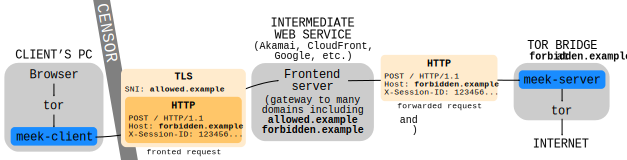
\includegraphics[width=\linewidth]{architecture}
\caption{
System architecture.
The Google frontend server is the server that dispatches requests to different services depending on the Host header.
Components that are new in our system are outlined in blue.
The ``Google infrastructure'' block may be replaced by other infrastructure that supports domain fronting.
}
\label{fig:architecture}
\end{figure*}

The main technical challenge in making this system work
is in encoding a TCP stream as a sequence of HTTP requests and responses.
\meekserver\ handles many clients at once, and their data streams
are split across multiple HTTP transactions.
In TCP, different streams are distinguished by their
(source~IP, source port, dest~IP, dest~port) tuple,
but we cannot do that because streams are split across multiple TCP sessions.
Rather, each instance of \meekclient\ generates at startup a random 32-byte
session ID, which is sent along with its requests in a special
X-Session-ID HTTP header.
\meekserver, when it sees a particular session ID for the first time,
opens up a new connection to the local Tor process,
and stores the session ID in a cache. Subsequent requests with the
same session ID will reuse the same Tor connection.
Entries are removed from the cache after a period of inactivity.

HTTP is fundamentally a pull-based protocol.
There is no way for the server to send data to the client without
the client first making a request.
The same applies to meek: when \meekserver\ has data to send back to
a client with a particular session ID, it cannot do so until it
receives a request from that client.
For this reason, \meekclient\ polls the server,
sending an empty request if necessary, every so often.
The polling interval starts short (100~ms) and grows exponentially
up to a maximum of 5~s.
Alternative techniques for push-like behavior,
such as HTTP long polling,
don't work well with App Engine,
because App Engine requires requests to finish within 60 seconds.

We implemented meek as a pluggable transport~\cite{pt} for Tor.
Although it is possible to use the system with proxies other than Tor,
using Tor has some attractive features.
The pluggable transports infrastructure makes it relatively easy to prototype
a circumvention technique and connect it to a global proxy network.
We can treat confidentiality and integrity of tunneled communication
as a problem solved by Tor, which we don't need to solve separately.
Tor's extra proxy hops mean that the HTTP reflector (App Engine)
and the entry bridge do not have to be trusted.

\section{Making the TLS handshake indistinguishable}
\label{sec:browserextension}

The practice of routing traffic through a web service with domain fronting
defeats both address-based blocking and active scanning.
The endpoint (which appears to be the front domain; e.g. www.google.com)
cannot be blocked because to block it would cause collateral damage.
Active scanning is defeated because if the censor accesses the same
domain as does the client, all they see is a web page served by the front domain.
Even though the censor knows some traffic is being fronted,
by looking only at IP addresses and domain names, it cannot determine which.

However, a savvy censor may also use content-based blocking
(deep packet inspection) as a basis for blocking.
Anything that reliably distinguishes meek's traffic from that of normal allowed traffic
(presumably web browsing) must be eliminated.
In this section we demonstrate how the client part of the TLS handshake can be used
to fingerprint different TLS implementations,
and how we use a web browser to camouflage meek's TLS.

There are many parts of the TLS handshake, but the two that
most distinguish the client are the list of ciphersuites and the
list of TLS extensions in the Client Hello.
Figure~\ref{fig:ciphersuites} shows how the list of ciphersuites
differs in different client implementations.
Figure~\ref{fig:ciphersuites:meek-client} is how our first prototype of \meekclient\ appeared on the wire,
using the built-in crypto/tls library of the Go programming language.
The list of ciphersuites is unlike that of a web browser,
and could be used as a fingerprint for blocking.
Tor itself was blocked by China in 2011 in exactly this way~\cite{bug4744}.
Similarly the list of TLS extensions (not shown)
differed between \meekclient\ and popular browsers.

\begin{figure}

\begin{subfigure}[t]{0.30\textwidth}
\begin{minipage}[t][17ex][t]{0.30\textwidth}
\tiny
\begin{verbatim}
TLS_ECDHE_RSA_WITH_AES_128_GCM_SHA256
TLS_ECDHE_ECDSA_WITH_AES_128_GCM_SHA256
TLS_ECDHE_RSA_WITH_RC4_128_SHA
TLS_ECDHE_ECDSA_WITH_RC4_128_SHA
TLS_ECDHE_RSA_WITH_AES_128_CBC_SHA
TLS_ECDHE_ECDSA_WITH_AES_128_CBC_SHA
TLS_ECDHE_RSA_WITH_AES_256_CBC_SHA
TLS_ECDHE_ECDSA_WITH_AES_256_CBC_SHA
TLS_RSA_WITH_RC4_128_SHA
TLS_RSA_WITH_AES_128_CBC_SHA
TLS_RSA_WITH_AES_256_CBC_SHA
TLS_ECDHE_RSA_WITH_3DES_EDE_CBC_SHA
TLS_RSA_WITH_3DES_EDE_CBC_SHA
\end{verbatim}
\end{minipage}
\caption{meek-client}
\label{fig:ciphersuites:meek-client}
\end{subfigure}
%
\begin{subfigure}[t]{0.30\textwidth}
\begin{minipage}[t][48ex][t]{0.30\textwidth}
\tiny
\begin{verbatim}
TLS_ECDHE_ECDSA_WITH_AES_256_CBC_SHA
TLS_ECDHE_ECDSA_WITH_AES_128_CBC_SHA
TLS_ECDHE_RSA_WITH_AES_128_CBC_SHA
TLS_ECDHE_RSA_WITH_AES_256_CBC_SHA
TLS_ECDHE_ECDSA_WITH_3DES_EDE_CBC_SHA
TLS_ECDHE_RSA_WITH_3DES_EDE_CBC_SHA
TLS_ECDHE_ECDSA_WITH_RC4_128_SHA
TLS_ECDHE_RSA_WITH_RC4_128_SHA
TLS_DHE_RSA_WITH_AES_128_CBC_SHA
TLS_DHE_DSS_WITH_AES_128_CBC_SHA
TLS_DHE_RSA_WITH_CAMELLIA_128_CBC_SHA
TLS_DHE_DSS_WITH_CAMELLIA_128_CBC_SHA
TLS_DHE_RSA_WITH_AES_256_CBC_SHA
TLS_DHE_DSS_WITH_AES_256_CBC_SHA
TLS_DHE_RSA_WITH_CAMELLIA_256_CBC_SHA
TLS_DHE_DSS_WITH_CAMELLIA_256_CBC_SHA
TLS_DHE_RSA_WITH_3DES_EDE_CBC_SHA
TLS_DHE_DSS_WITH_3DES_EDE_CBC_SHA
TLS_ECDH_ECDSA_WITH_AES_128_CBC_SHA
TLS_ECDH_RSA_WITH_AES_128_CBC_SHA
TLS_ECDH_ECDSA_WITH_AES_256_CBC_SHA
TLS_ECDH_RSA_WITH_AES_256_CBC_SHA
TLS_ECDH_ECDSA_WITH_3DES_EDE_CBC_SHA
TLS_ECDH_RSA_WITH_3DES_EDE_CBC_SHA
TLS_ECDH_ECDSA_WITH_RC4_128_SHA
TLS_ECDH_RSA_WITH_RC4_128_SHA
TLS_RSA_WITH_AES_128_CBC_SHA
TLS_RSA_WITH_CAMELLIA_128_CBC_SHA
TLS_RSA_WITH_AES_256_CBC_SHA
TLS_RSA_WITH_CAMELLIA_256_CBC_SHA
TLS_RSA_WITH_SEED_CBC_SHA
SSL_RSA_FIPS_WITH_3DES_EDE_CBC_SHA
TLS_RSA_WITH_3DES_EDE_CBC_SHA
TLS_RSA_WITH_RC4_128_SHA
TLS_RSA_WITH_RC4_128_MD5
\end{verbatim}
\end{minipage}
\caption{Firefox 24}
\label{fig:ciphersuites:firefox}
\end{subfigure}
%
\begin{subfigure}[t]{0.30\textwidth}
\begin{minipage}[t][27ex][t]{0.30\textwidth}
\tiny
\begin{verbatim}
TLS_ECDHE_ECDSA_WITH_AES_128_GCM_SHA256
TLS_ECDHE_RSA_WITH_AES_128_GCM_SHA256
TLS_DHE_RSA_WITH_AES_128_GCM_SHA256
TLS_ECDHE_ECDSA_WITH_CHACHA20_POLY1305_SHA256
TLS_ECDHE_RSA_WITH_CHACHA20_POLY1305_SHA256
TLS_RSA_WITH_AES_128_GCM_SHA256
TLS_ECDHE_ECDSA_WITH_AES_256_CBC_SHA
TLS_ECDHE_RSA_WITH_AES_256_CBC_SHA
TLS_DHE_RSA_WITH_AES_256_CBC_SHA
TLS_RSA_WITH_AES_256_CBC_SHA
TLS_ECDHE_ECDSA_WITH_RC4_128_SHA
TLS_ECDHE_ECDSA_WITH_AES_128_CBC_SHA
TLS_ECDHE_RSA_WITH_RC4_128_SHA
TLS_ECDHE_RSA_WITH_AES_128_CBC_SHA
TLS_DHE_RSA_WITH_AES_128_CBC_SHA
TLS_DHE_DSS_WITH_AES_128_CBC_SHA
TLS_RSA_WITH_RC4_128_SHA
TLS_RSA_WITH_RC4_128_MD5
TLS_RSA_WITH_AES_128_CBC_SHA
TLS_RSA_WITH_3DES_EDE_CBC_SHA
\end{verbatim}
\end{minipage}
\caption{Chrome 33}
\label{fig:ciphersuites:chrome}
\end{subfigure}

\caption{Differences in ciphersuites offered by
our \meekclient\ program when it accesses the network directly,
and by two web browsers.
The distinctive ciphersuites offered by \meekclient\ can be used as part of a blocking fingerprint.
As a remedy we have \meekclient\ proxy its TLS through a web browser extension.
}
\label{fig:ciphersuites}
\end{figure}

In response to the threat of TLS fingerprinting,
we modified \meekclient\ to proxy its HTTP requests through a local web browser extension.
\meekclient\ tells the extension what URLs to fetch, and the extension fetches them.
The TLS fingerprint looks like that of a browser, because it is that of a browser.
We implemented two versions of the extension, one for Firefox and one for Chrome.
They work similarly: they open a TCP port on localhost,
await instructions from \meekclient\ on what HTTP requests to make,
issue the requests, and return the responses.

\begin{figure}
\centering
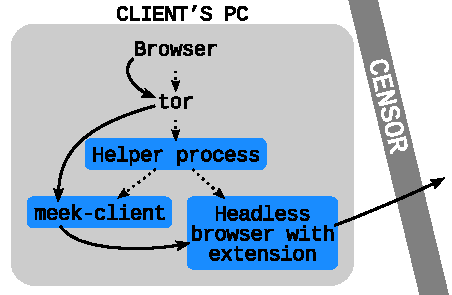
\includegraphics[height=1.5in]{browser-architecture}
\caption{
Client architecture including a browser extension for TLS camouflage.
Dashed lines show the process hierarchy.
Solid lines show the flow of outgoing communication.
The headless instance of the browser runs in the background and is invisible to the user.
This figure is a detailed view of the ``User's PC'' component of Figure~\ref{fig:architecture}.
}
\label{fig:browser-architecture}
\end{figure}

Figure~\ref{fig:browser-architecture} shows the interaction of components
on the user's computer.
Rather than starting \meekclient\ as a pluggable transport directly, the Tor
process starts a helper process that starts both \meekclient\
and a headless browser instance.
The headless browser runs our extension in a separate
process and separate browser profile from the browser the
user interacts with; the two browser instances share no state.
\meekclient\ is configured to issue its requests through the browser extension;
in this configuration, the headless browser is the only thing that ever touches the network.
When run with a browser extension, meek has the same TLS signature
as Firefox (Figure~\ref{fig:ciphersuites:firefox}) or
Chrome (Figure~\ref{fig:ciphersuites:chrome}).

The use of a browser extension offers benefits beyond its TLS signature.
We inherit other characteristics of the browser:
how often it resolves DNS names,
its connection reuse,
and HTTP keepalive behavior.
The Firefox extension has special usability advantages because the Tor Browser Bundle
uses a modified Firefox.
We can include a small extension in the browser bundle, reusing the existing
Firefox executable, without increasing the download size of the bundle much,
and without requiring users to separately configure a browser to run the extension.

The development of the browser extensions posed some unexpected challenges.
Tor Browser disables TLS session tickets because they can be used as linking identifiers,
but the lack of session tickets shows up as a missing TLS extension,
so we had to reenable them in the headless browser.
(Doing so doesn't harm Tor Browser's anonymity:
if session tickets are used, they are used only on the circumvention layer
between the user and the frontend server. Tor Browser's own TLS is tunneled
within the circumvention layer, and session tickets are still disabled at that level.)
The Chrome extension needed to be split into two pieces, an extension and an app,
because an extension cannot open a listening socket and an app cannot make HTTP requests.

\section{Camouflage of traffic characteristics}
\label{sec:trafficstatistics}

The censor cannot sniff the content of communications or infer the usage of meek 
from packet \emph{data}, 
since the communication is encrypted inside the TLS session, and we have devoted large efforts 
in hiding TLS handshake fingerprints. However, it is still possible that the censor can detect 
the existence of meek according to the \emph{meta-data}, i.e. traffic characteristics. 
In this section we study a collection of traffic characteristics and evaluate their possibilities of becoming
the censor's interest. Specifically, we consider three characteristics: 1) payload length of
TCP packets, 2) number of concurrent HTTPS connections, 3) HTTPS connection lifetime. 

To collect the traffic trace of meek, we browses the Alexa top 500 websites sequentially using 
the Tor Browser Bundle and dump the traffic trace from the network interface. We ensured only
the browser can successfully access the network by setting
up the \texttt{iptables} firewall so that packets from other processes will be dropped. We also 
obtain a 10-minute sample of normal HTTPS traffic trace from LBL. The trace is 983 MB in total. 
We also specifically extracted the traffic between LBL and Google from the trace. Since the trace 
only has packet headers, we cannot extract the domain information. However, the \texttt{TXT} DNS
records of the domain \texttt{\_netblocks.google.com} shows the IP address blocks that belongs to
Google. Therefore, we determine whether a flow is from or to Google by examining the address in the 
IP header. We only interested in the Google traffic only, because the censor who wants to defeat meek
will be mostly likely to compare suspicious traffic with normal Google traffic. The size of the 
Google trace is 312 MB. 


\begin{figure}
\centering
\begin{subfigure}[b]{0.5\textwidth}
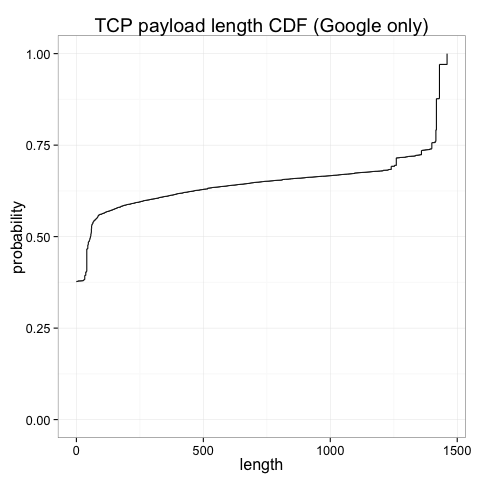
\includegraphics[width=\textwidth]{figs/datalen-google-cdf.png}
\caption{Normal Google Traffic}
\label{fig:len:lbl}
\end{subfigure}%
%add desired spacing between images, e. g. ~, \quad, \qquad, \hfill etc.
%(or a blank line to force the subfigure onto a new line)
\begin{subfigure}[b]{0.5\textwidth}
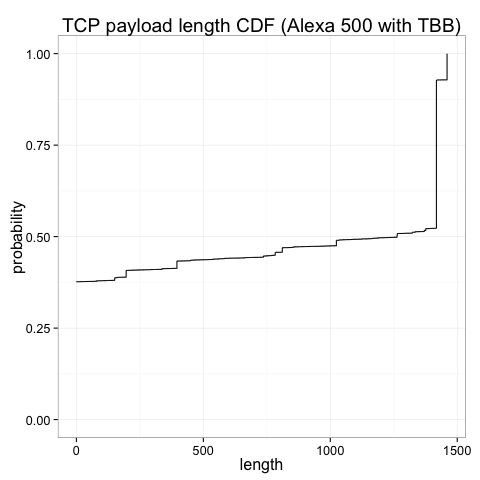
\includegraphics[width=\textwidth]{figs/datalen-tbb-cdf.png}
\caption{Traffic Using meek}
\label{fig:len:meek}
\end{subfigure}

\caption{TCP packet payload size distribution}
\label{fig:len}
\end{figure}

\paragraph{TCP payload length}
Figure ~\ref{fig:len} shows the payload size distribution of normal traffic and meek's traffic. Both
figures exhibit a significant amount of packets with no payload. These packets are mostly TCP SYN and ACK
packets. Figure ~\ref{fig:len:lbl} shows the distribution of normal traffic, which indicates a large portion
of small-sized packets. However, in the meek's traffic shown in Figure ~\ref{fig:len:meek}, most packets
are large packets ranging from 1400 bytes to 1500 bytes. This result is unexpected, because the underlying packets 
in the TLS session are sent from Tor. By default, each Tor cell is 512 bytes, but meek changes the packet size 
distribution. Therefore, meek provides traffic shaping without additional efforts.

To explain the phenomenon, recall that we use browsers to handle HTTPS connections for meek in order
to hide TLS handshake characteristics.
Browsers also apply techniques like HTTP pipelining to improve performance. Since meek is always communicating with
the same Google frontend server, the browser will keep the persistent TLS connection. In addition, small requests 
can be batched into a large chunk before being sent. This explains why large packets are mostly seen from the trace that
records meek's traffic.
In contract, normal users may not have persistent connections to Google. For example, a user may search a keyword on
Google, click a result, and then close the tab that displays search results. The browser may close the 
connection immediately after the user leaves the Google web page. Next time the user browses Google search, the browser 
opens a new connection. In this case, small requests do not have such opportunity for batching.

These browser techniques improve performance, but also pose unexpected consequences. 
Although meek alters the packet size distribution of underlying Tor traffic, 
the censor may be aware of the distribution of meek itself. 
Additionally, the persistent connection itself can be an issue.
We thus investigated other related characteristics.

\begin{figure}
\centering
\includegraphics[width=0.7\textwidth, angle=270]{figs/connections-google.eps}
\caption{Histogram of each user's connections in the 10-minute window}
\label{fig:connections}
\end{figure}
%add desired spacing between images, e. g. ~, \quad, \qquad, \hfill etc.
%(or a blank line to force the subfigure onto a new line)
\begin{figure}
\centering
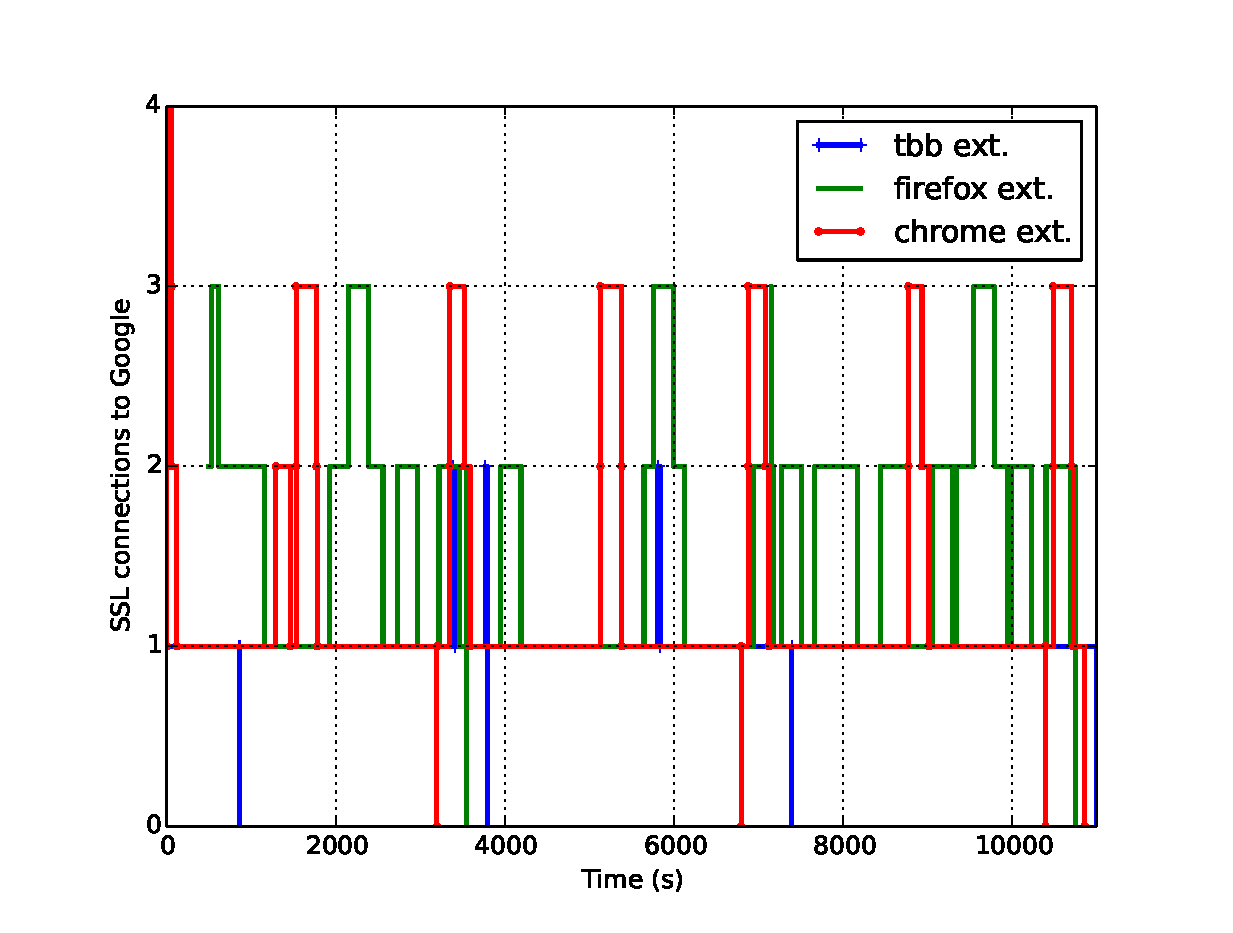
\includegraphics[width=0.8\textwidth]{figs/conns.eps}
\caption{Concurrent HTTPS connections over time. We measure the trace for the Tor Browser Bundle and Firefox/Chrome extensions.}
\label{fig:conconns}
\end{figure}

\paragraph{Concurrent connections}
Figure ~\ref{fig:connections} shows how many HTTPS connections to Google did a user make 
during the 10-minute measurement window.
There are 34,732 connections in total from 2,745 unique IPs. We observe that the majority of users have less than 
50 connections to the Google frontend server, and most of the numbers concentrate on 1 ~ 10. This is not unexpected
because a typical pattern of using Google is using the Google search as a stepping stone for other websites.

We measure the number of concurrent HTTPS connections during the automated browsing of Alexa
top 500 sites using three platforms: Tor Browser Bundle, Safari + Firefox extension, and Safari + Chrome extension.
Figure ~\ref{fig:conconns} shows the number over time. We can see that most of the time
the browser has one HTTPS connection to Google. Sometimes the browser may have more than one connection
due to background activities such as statistics reporting. In all cases the number of connections is always 
less than 5. We can conclude that the number of concurrent connections does not show distinct characteristics, as 
a small number of connections can be considered as a normal behavior.

\begin{figure}
\centering
\begin{subfigure}[b]{0.5\textwidth}
\includegraphics[height=\textwidth, angle=270]{figs/flowduration-google-cdf.eps}
\caption{Normal Google Traffic}
\label{fig:duration:lbl}
\end{subfigure}%
%add desired spacing between images, e. g. ~, \quad, \qquad, \hfill etc.
%(or a blank line to force the subfigure onto a new line)
\begin{subfigure}[b]{0.5\textwidth}
\includegraphics[height=\textwidth, angle=270]{figs/flowduration-tbb-cdf.eps}
\caption{Traffic Using meek (Notice the x-axis)}
\label{fig:duration:meek}
\end{subfigure}

\caption{Connection lifetime distribution}
\label{fig:duration}
\end{figure}

\paragraph{Connection lifetime}
We consider the connection lifetime as a potential weakness. Figure ~\ref{fig:duration:lbl} shows the 
connection lifetime distribution of normal traffic. Interestingly we can see the concentration on 
several discrete values: 60s, 120s, 180s, 240s. We hypothesize that it is due to the HTTP Keep-Alive 
timeout of different browsers and web services. Another important observation is the concentration on 
durations that exceed 600 seconds. Note that our trace only contains 10 minutes' data, therefore the concentration 
on 600 seconds does not reflect that these connections' actual duration is 600 seconds. Rather, 600 seconds
is the lower bound of their actual duration. Thus, we can conclude that only about 10\% connections last 
longer than 600 seconds.

The distribution of meek's traffic, in contrast, is totally different. First, there are much fewer connections, which is 
consistent with the discussions above. Second, the durations are much longer if we notice the x-axis in Figure ~\ref{fig:duration:meek}. If there is not a case in which normal users also have such long connections when browsing Google, the 
censor can potentially block any long connections between users and Google. Even if this is the case, the
censor has to wait until a time threshold is reached. The user might have already obtained the forbidden data she wants, or 
meek could simply restart a connection.

\paragraph{Conclusion} So far we do not find any obvious traffic characteristics that can be useful for
distinguishing meek's traffic. But admittedly there two potential weaknesses: long-lived connections 
with bulk data transfer, and deviated distribution of packet sizes. To fundamentally fix these weaknesses 
we need to transform to the traffic into the normal-looking traffic. The problem is inherently difficult, because we need to know \emph{what} is normal traffic, i.e. what is the model of normal traffic, which is an open problem. However, 
the arm-race game is symmetric; since finding a right model is a difficult task for us, it is also difficult for 
the censor. Therefore, the censor can only find ad-hoc features to block forbidden traffic, which are relatively 
easy to defend against. 

\section{Security}

Domain fronting shares a weakness with decoy routing,
which is that the overt and covert destinations lie on different
network paths.
The difference in paths may create side channels---latency measurements for instance---that
enable the censor to
distinguish fronted traffic from traffic that is truly destined
to the front domain.
For example, a CDN can be expected to have responses
to some fraction of requests already in cache,
and respond to those requests with low latency.
Fronted traffic, on the other hand, always continues all the way
to the origin server after reaching the CDN (as if nothing were ever cached),
resulting in a higher latency.
Latency measurement was applied to decoy routing by Schuhard et~al.~\cite[Section~5]{ccs2012-decoys},
who compared empirical round-trip-time distributions using a
Kolmogorov--Smirnov test.
% time between ChangeCipherSpec and ApplicationData

When domain fronting is combined with Tor,
the CDN or web service effectively becomes
what Tor calls a ``guard node,''
a host with a privileged network position that can observe
the ciphertext entering the network.
One consequence of this fact is that Google (for example)
knows the IP addresses of everyone using the circumvention system,
just as if it were those users' ISP.
Another consequence is that the CDN or web service gets
to observe and correlate both entry and exit traffic,
in the special case where the target of the communication
also lies on the same CDN or web service.
For example, a user fronting through App Engine and
browsing YouTube reveals both their entry and exit traffic to Google,
which may attempt through traffic analysis to determine
which entry packets correspond to which exit packets.
The problem is hard to counter, because the front domain needs
to be a popular destination in order to have high collateral damage,
but popular destinations by definition tend to be visited a lot.
% Possible countermeasure is traffic fingerprinting resistance
% like what mjuarez is working on, mostly orthogonal to circumvention.

% Edge servers within the censored region.
% Censor could block on the way to the origin server,
% if the censor has visibility to it.
% Maybe the CDN has its own private high-speed cables,
% or it VPNs its own stuff or something.

% Firefox plugin uses normal browser trust store.
% Adversary controls CAs. Can MITM and read your tag and block you.
% Maybe not willing to risk getting caught in MITM.
% Could conceivably send cover traffic if MITM detected, but blah.

\section{Deployment}
\label{sec:deployment}

We implemented meek as a Tor pluggable transport~\cite{pt}
and built experimental releases of the Tor Browser Bundle featuring meek.
The browser bundle includes Tor and a version of Firefox
called Tor Browser that is patched to defend against application-layer identity leaks.
Users need to download and run the bundle and select meek from the list of transports,
and then a browser window appears,
configured to use meek for circumvention and Tor for anonymity.
We announced our prototype bundles on Tor development mailing lists,
and from there they were picked up by Tor Weekly News on the Tor blog.

\begin{figure}
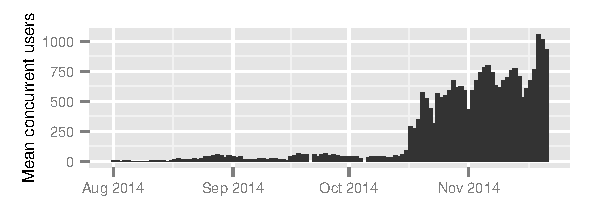
\includegraphics[width=\linewidth]{clients-meek}
\caption{Number of concurrent users using the meek transport,
as reported by the Tor Metrics Portal.}
\label{fig:clients}
\end{figure}

Figure~\ref{fig:clients} shows the number of concurrent users of meek between January and May~2014,
as reported by the Tor Metrics Portal~\cite{metrics-meek}.
The number of concurrent users is estimated by counting directory requests made over the transport~\cite{counting-daily-bridge-users}.
The drop to zero on May~8 coincides with the reinstallation of the Tor bridge used by meek.

We are running a paid instance of the web app on App Engine for use by the public.
The cost for bandwidth on App Engine is \$0.12 per gigabyte,
with one gigabyte free each day.
The total cost has so far been \$1.11, with bills of
\$0.09 in March,
\$0.73 in April,
and \$0.29 in the first half of May.

meek has a home page at
\url{https://trac.torproject.org/projects/tor/wiki/doc/meek}.
Our source code is in the Git repository at
\url{https://git.torproject.org/pluggable-transports/meek.git}.
As of version 0.5 (May~7, 2014), the source code consists of
about 800 lines of Go for the client programs,
400 lines for \meekserver, and
100 lines for the reflector web app.
Each of the browser extensions
(one for Firefox, one for Chrome)
is about 300 lines of JavaScript.

% Psiphon

\subsection{Other deployment scenarios}
\label{sec:otherdeployment}

The deployment we envision and have started to implement
uses a single paid App Engine instance, which is publicly known and usable by anyone.
Client software is configured to use this public instance by default.
A preconfigured public instance has great usability advantages
because there is nothing for the user to upload and nothing to configure.
The number of parties able to analyze users' traffic patterns is somewhat increased:
the path from user to Tor bridge now includes App Engine and the web app operators,
in addition to the ISP and intermediate routers that were there before.
On the other hand, the Tor bridge no longer gets to see users' IP addresses:
all it sees are many connections from App Engine.

Users are also free to upload their own personal copy of the App Engine code, as is done with GoAgent.
App Engine imposes bandwidth quotas on unpaid apps, but they are high enough to allow daily web browsing.
In this scenario, Google still has a privileged network position,
but the user's traffic patterns are no longer visible to the operators of a public app instance.
% Outgoing HTTP requests include app id? As good as an IP address.

A censor can block meek by blocking access to Google entirely,
but other systems can take the place of Google.
An attractive alternative is CloudFlare, a large content delivery network,
which supports domain fronting, dispatching requests based on the Host header
rather than IP or SNI.
We did not test deployment on CloudFlare,
because their terms of service are not clear on whether this kind of use is allowed,
and we got an ambiguous answer when we asked for clarification.
A particular concern when using CloudFlare or other content delivery networks is the choice of front domain.
If one domain is being used particularly as a front for circumvention traffic,
it may find itself blocked by the censor, even though it is not itself
involved in any circumvention.
One good solution to this problem may be not to use a domain name at all,
but only the IP address of one of CloudFlare's servers.
The censor will then face the choice of allowing circumvention traffic,
or else blocking a large number of unrelated web sites.

% We were not able to make the system work with Amazon CloudFront nor Akamai.
% Dreamhost? Other HTTPS webhosts with PHP bridge?

The code that runs on App Engine is very simple.
It just statelessly copies HTTP requests and responses.
Another possible deployment scenario uses a PHP implementation of the reflector,
deployed on an ordinary web hosting service other than App Engine.
In this scenario, domain fronting is not used;
instead unblockability depends on there being many (individually blockable) PHP reflectors.
In other words, it is roughly the same situation as exists today with Tor bridges,
except that it can be much easier for a volunteer to upload a PHP file to a web host
than to set up Tor bridge.
Such PHP bridges could potentially automatically report their own URLs,
which could be distributed using a system like BridgeDB.

\section{Future work}

In future work we would like to implement pipelining of requests,
so that more than one HTTP request can be outstanding at a time.
This would have better performance compared to the current system,
which serializes requests and responses in order to keep the
underlying TCP stream in order.
A system of sequence numbers and acknowledgments as used in OSS~\cite{oss}
could make this possible.
% Would be useful for Iran-like session cutoff, independent of meek.

% Performance measurements
We would like to do more quantitative performance measurements,
in order to measure the overhead in bandwidth and latency that meek has over plain Tor.
We have done informal tests, such as browsing YouTube,
but have not yet put numbers to our measurements.

% Load balancing

\section*{Acknowledgments}

We thank Vern Paxson, Nick Weaver, and Doug Tygar for inspiring conversation on this topic.
Special thanks go to the members of the tor-qa and tor-dev mailing lists
who responded to our design ideas, reviewed source code, and tested our prototypes.
% George Kadianakis
% Georg Koppen
% Lunar
% Yawning Angel
% Rod Hynes and Michael Hull of Psiphon.
% Johanna Amann for getting the fraction of SNI from ICSI notary:
%   https://trac.torproject.org/projects/tor/ticket/12208#comment:5

%%%%%%%

% HTTPS or not on the App Engine--bridge link.
% HTTPS obscures session ids, equivalent to obscuring TCP connections in other transports.
% Increases latency a lot: \approx 100 ms increased to \approx 350 ms when I tried it in March 2014.

\bibliographystyle{IEEEtran}
\bibliography{meek}

\end{document}
